\section{Обзор}
Предлагаемый в данной работе алгоритм заимствует распространённые принципы существующих работ данной области. Помимо этого переиспользуется RNGLR-алгоритм синтаксического анализа вместе с соответствующими структурами данных. В данном разделе приведён обзор подходов к анализу встроенных языков, дано краткое описание RNGLR-алгоритма, а также описан проект, в рамках которого велась разработка предложенного алгоритма.

\subsection{Подходы к анализу динамически формируемых выражений}
Анализ встроенных языков начинается с поиска и выделения в исходном коде основной программы так называемых \emph{точек интереса} или \emph{хотспотов} (hotspot), в которых осуществляется исполнение или передача формируемого выражения выделенной компоненте. Определение точек интереса обычно производится либо с помощью пользователя, посредством аннотаций или явного указания соответствующих строк исходного кода, либо автоматически, если есть некоторые знания об используемом фреймворке. Например, на хотспот могут указывать такие функции как \textsc{exec} динамического SQL. В точке интереса производится вычисление множества значений динамически формируемого выражения, а также его последующая аппроксимация. Следующим шагом, как правило, производится токенизация, то есть по языку над алфавитом символов строится язык над алфавитом терминалов эталонной грамматики. Затем полученный язык может анализироваться (синтаксически и семантически) в зависимости от стоящей задачи. Перечисленные шаги не обязательно производятся последовательно, более того, некоторые из них могут быть опущены. 

Под \emph{регулярной аппроксимацией} мы подразумеваем аппроксимирование множества значений динамически формируемого выражения некоторым регулярным выражением. В терминах, привычных для задач распознавания, проверка корректности выражений из аппроксимирующего множества формулируется как задача проверки включения регулярного языка в эталонный, как правило, контекстно-свободный, язык, которая разрешима во многих важных на практике случаях~\cite{LangInclusion}. Многие существующие работы по анализу встроенных языков используют такой подход. В работе~\cite{Stranger} для построения аппроксимации используется анализ прямой достижимости (forward reachability analysis), дальнейший анализ основан на распознавании образцов (pattern detection) в аппроксимирующем множестве или генерации некоторого конечного подмножества строк для анализа с помощью отдельных инструментов. В работе~\cite{JSA} построение регулярной аппроксимации осуществляется посредством расширения контекстно-свободной аппроксимации, построенной во время анализа исходного кода основной программы. Предложенный нами подход вдохновлён проектом Alvor~\cite{Alvor,Alvor2}, который использует технику, основанную на GLR-алгоритме, для синтаксического анализа регулярной аппроксимации. В данном проекте для упрощения задачи синтаксического анализа, регулярный язык над алфавитом символов сначала трансформируется в регулярный язык над алфавитом терминалов эталонной грамматики с помощью специальной процедуры лексического анализа. 

В серии работ~\cite{AbstrParsing,LRAbstrParsing,LRAbstrParsingSema} предложен подход, основанный на явном представлении множества формируемых выражений в виде системы уравнений потока данных (data-flow equations). В качестве базы алгоритма синтаксического анализа выбран традиционный LALR(1)-алгоритм, при этом переиспользуются таблицы управления. Синтаксический анализ производится во время решения уравнений потока данных в домене абстрактных стеков. Проблема возможного бесконечного роста стеков, возникающая в общем случае, разрешается с помощью абстрактной интерпретации (abstract interpretation~\cite{AbstractInterpretation}). Впоследствии данный подход был расширен вычислением семантики с помощью атрибутных грамматик, что позволило анализировать более широкий, чем LALR(1), класс грамматик. 

\subsection{RNGLR-алгоритм}
RNGLR-алгоритм (Right-Nulled Generalized LR) является модификацией предложенного Масару Томитой алгоритма Generalized LR (GLR)~\cite{Tomita}, предназначенного для анализа естественных языков. GLR-алгоритм был предназначен для анализа неоднозначных контекстно-свободных грамматик. Неоднозначности грамматики порождают конфликты сдвиг/свёртка (shift/reduce) и свёртка/свёртка (reduce/reduce). GLR-алгоритм использует управляющие таблицы, схожие с управляющими таблицами LR-алгоритма, ячейки которых могут содержать несколько действий. Основная идея GLR-алгоритма состоит в проведении всех возможных действий во время синтаксического анализа. При этом для эффективного представления множества стеков и деревьев вывода используются особые структуры данных, основанные на графах.

Оригинальный алгоритм, предложенный Томитой, не был способен анализировать все контекстно-свободные грамматики. Элизабет Скотт и Адриан Джонстоун предложили RNGLR-алгоритм, который расширяет GLR-алгоритм специальным способом обработки обнуляемых справа правил (right-nullable rules, имеющих вид $\mathrm{A} \rightarrow \alpha \beta$, где $\beta$ выводит пустую строку $\epsilon$).

\begin{algorithm}[!ht]
\begin{algorithmic}[1]
\caption{RNGLR-алгоритм}
\label{rnglr}
\Function{parse}{$grammar, input$}
  \State{$\mathcal{R} \gets \emptyset$} \Comment{Очередь троек: вершина GSS, нетерминал, длина свёртки}
  \State{$\mathcal{Q} \gets \emptyset$} \Comment{Коллекция пар: вершина GSS, состояние парсера}
  \If{$input = \epsilon$}
    \If{$grammar$ accepts empty input} {report success}
    \Else { report failure}
    \EndIf
  \Else
    \State{\Call{addVertex}{$0, 0, startState$}}
    \ForAll{$i$ in $0..input.Length-1$}
      \State{\Call{reduce}{$i$}}
      \State{\Call{push}{$i$}}
    \EndFor
    \If{$i=input.Length-1$ and there is a vertex in the last level of GSS which state is accepting}
      \State{report success}
    \Else { report failure}
    \EndIf
  \EndIf
\EndFunction
\Function{reduce}{$i$}
  \While{$\mathcal{R}$ is not empty}
    \State{$(v, N, l) \gets \mathcal{R}.Dequeue()$}
    \State{find the set $\mathcal{X}$ of vertices reachable from $v$ along the path of length $(l-1)$}
    \State{or length $0$ if $l=0$}
    \ForAll{$v_{h} = (level_{h}, state_{h})$ in $\mathcal{X}$}
      \State{$state_{t} \gets$ calculate new state by $state_{h}$ and nonterminal $N$}
      \State{\Call{addEdge}{$i, v_{h}, v.level, state_{tail}, (l=0)$}}
    \EndFor
  \EndWhile
\EndFunction
\Function{push}{$i$}
  \State{$\mathcal{Q^{'}} \gets$ copy $\mathcal{Q}$}
  \While{$\mathcal{Q^{'}}$ is not empty}
    \State{$(v, state) \gets \mathcal{Q}.Dequeue()$}
    \State{\Call{addEdge}{$i, v, v.level + 1, state, false$}}
  \EndWhile
\EndFunction
\end{algorithmic}
\end{algorithm}

\begin{algorithm}[!ht]
\begin{algorithmic}[1]
\caption{Построение GSS}
\label{RNGLRMain}
\Function{addVertex}{$i, level, state$}
  \If{GSS does not contain vertex $v = (level, state)$}
    \State{add new vertex $v = (level, state)$ to GSS}
    \State{calculate the set of shifts by $v$ and the $input[i+1]$ and add them to $\mathcal{Q}$}
    \State{calculate the set of zero-reductions by $v$ and the $input[i+1]$ and}
    \State{add them to $\mathcal{R}$}
  \EndIf
  \State{\Return{$v$}}
\EndFunction
\Function{addEdge}{$i, v_{h}, level_{t}, state_{t}, isZeroReduction$}
  \State{$v_{t} \gets$ \Call{addVertex}{$i, level_{t}, state_{t}$}}
  \If{GSS does not contain edge from $v_{t}$ to $v_{h}$}
    \State{add new edge from $v_{t}$ to $v_{h}$ to GSS}
    \If{not $isZeroReduction$}
      \State{calculate the set of reductions by $v$ and the $input[i+1]$ and}
      \State{add them to $\mathcal{R}$}
    \EndIf
  \EndIf
\EndFunction
\end{algorithmic}
\end{algorithm}

Для эффективного представления множества стеков во время синтаксического анализа в алгоритме RNGLR используется структурированный в виде графа стек (Graph Structured Stack, GSS), который является ориентированным графом, чьи вершины соответствуют  элементам отдельных стеков, а ребра связывают последовательные элементы. Каждая вершина может иметь несколько входящих рёбер, что соответствует слиянию нескольких стеков, за счёт чего производится переиспользование общих участков отдельных стеков. Вершина GSS~--- это пара $(s,l)$, где $s$~--- состояние парсера, а $l$~--- уровень (позиция во входном потоке).

RNGLR-алгоритм последовательно считывает символы входного потока слева направо, по одному за раз, и строит GSS по "слоям": сначала осуществляются все возможные свёртки для данного символа, после чего сдвигается следующий символ со входа. Свёртка или сдвиг модифицируют GSS следующим образом. Предположим, что необходимо добавить ребро $(v_t,v_h)$ в GSS. По построению, конечная вершина добавляемой дуги к такому моменту уже обязательно находится в GSS. Если начальная вершина также содержится в GSS, то в граф добавляется новое ребро (если оно ранее не было добавлено), иначе создаются и добавляются в граф и начальная вершина, и ребро. Каждый раз, когда создаётся новая вершина $v=(s,l)$, алгоритм вычисляет новое состояние парсера $s'$ по $s$ и следующему символу входного потока. Пара $(v,s')$, называемая push, добавляется в глобальную коллекцию $\mathcal{Q}$. Также при добавлении новой вершины в GSS вычисляется множество $\epsilon$-свёрток, после чего элементы этого множества добавляются в глобальную очередь $\mathcal{R}$. Свёртки длины $l>0$ вычисляются и добавляются в $\mathcal{R}$ каждый раз, когда создаётся новое (не-$\epsilon$) ребро. Подробное описание работы со структурированным в виде графа стеком GSS содержится в алгоритме~\ref{RNGLRMain}.

В силу неоднозначности грамматики входная строка может иметь несколько деревьев вывода, как правило, содержащих множество идентичных поддреревьев. Для того, чтобы компактно хранить множество деревьев вывода, создано компактное представление леса разбора (Shared Packed Parse Forest, SPPF)~\cite{SPPF}. SPPF является ориентированным графом и обладает следующей структурой.
\begin{enumerate}
  \item \emph{Корень} (то есть, вершина, не имеющая входящих дуг) соответствует стартовому нетерминалу грамматики.
  \item \emph{Терминальные} вершины, не имеющие исходящих дуг, соответствуют либо терминалам грамматики, либо деревьям вывода пустой строки $\epsilon$.
  \item \emph{Нетерминальные} вершины являются корнем дерева вывода некоторого нетерминала грамматики; только вершины-продукции могут быть непосредственно достижимы из таких вершин.
  \item \emph{Вершины-продукции}, представляющие правую часть правила грамматики для соответствующего нетерминала. Вершины, непосредственно достижимые из них, упорядочены и могут являться либо терминальными, либо нетерминальными вершинами. Количество таких вершин лежит в промежутке $[l-k..l]$, где $l$~--- это длина правой части продукции, а $k$~--- количество финальных символов, выводящих $\epsilon$ (правые обнуляемые символы игнорируются для уменьшения потребления памяти).
\end{enumerate}

SPPF создаётся одновременно с построением GSS. Каждое ребро GSS ассоциировано с либо с терминальным, либо с нетерминальным узлом. Когда добавление ребра в GSS происходит во время операции push, новая терминальная вершина создаётся и ассоциируется с ребром. Нетерминальные вершины ассоциируются с ребрами, добавленными во время операции reduce. Если ребро уже было в GSS, к ассоциированной с ним нетерминальной вершине добавляется новая вершина-продукция. Подграфы, ассоциированные с рёбрами пути, вдоль которого осуществлялась свёртка, добавляются как дети к вершине-продукции. После того, как входной поток прочитан до конца, производится поиск всех вершин, имеющих принимающее состояние анализатора, после чего подграфы, ассоциированные с исходящими из таких вершин рёбрами, объединяются в один граф. Из полученного графа удаляются все недостижимые из корня вершины, что в итоге оставляет только корректные деревья разбора для входной строки. 

Алгоритм~\ref{rnglr} представляет более детальное описание алгоритма.

\subsection{Проект YaccConstructor и платформа для анализа встроенных языков}
В рамках проекта YaccConstructor~\cite{YC} лаборатории языков инструментов JetBrains на математико-механическом факультете СПбГУ проводятся исследования в области лексического и синтаксического анализа, а также статического анализа встроенных языков. Проект YaccConstructor представляет собой модульный инструмент, имеет собственный язык спецификации грамматик, объединяет различные алгоритмы лексического и синтаксического анализа. В рамках проекта была создана платформа для статического анализа встроенного кода~\cite{SECR14}; диаграмма последовательности, иллюстрирующая взаимодействие модулей платформы представлена на рисунке~\ref{seq}. Цветом выделена компонента, осуществляющая синтаксический анализ множества значений динамически формируемого выражения. 
\begin{figure}[!h]
 \centering
 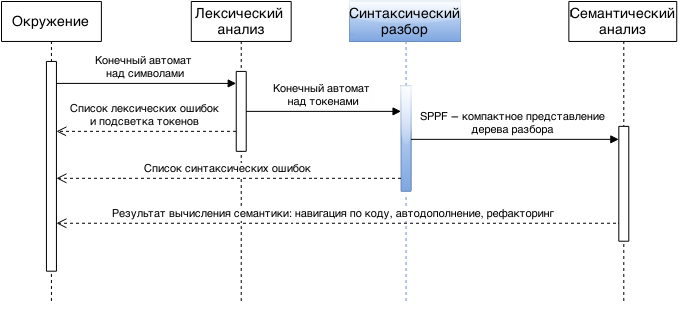
\includegraphics[width=15cm]{pics/Seq_rus.png}
 \caption{Диаграмма последовательности: взаимодействие компонентов
инструмента YaccConstructor}
 \label{seq}
\end{figure}

Предыдущая реализация платформы работала с грубой аппроксимацией, которая не осуществляла поддержку формирования выражения в циклах и с помощью строковых выражений~\cite{SECR13}. Используемая аппроксимация не являлась аппроксимацией сверху, что сказывалось на точности результатов анализа, и поэтому впоследствии она была заменена на регулярную. Однако это повлекло необходимость изменения алгоритма синтаксического анализа, чему и посвящена данная работа. 